\section{Contract Transactions}
\label{section:contract_transactions}

\subsection{Mechanism}

\begin{figure}[H]
\centering
\includegraphics[scale=0.60]{07_contract_transactions/png/contract_transaction}
\caption{Contract Transactions}
\label{fig:contract_transaction}
\end{figure}

\subsection{Negative Feedback}

There are two money transfers in a contract transaction. The first is a transfer of money in
exchange for a good. As with time transactions, interest rates are prices and are subject to
excess supply/excess demand response.

\subsection{Positive Feedback}

A positive feedback can occur if people believe that they can resell something at a later time
with a higher price. This may increase demand rather than reduce it as in the negative feedback
case.  This can occur with both exchange transactions and time transactions if the price of a good
is increasing over time. We'll look at the proces in \ref{section:other_transactions}. Land and
precious metals sometimes behave like this. We'll look at the proces in
\ref{section:other_transactions}.
 
\subsection{Proxy Accounts}

Contract transactions can be used to construct proxy accounts such as bank accounts, that are
external to the accounts of the digital currency.

\begin{figure}[H]
\centering
\includegraphics[scale=0.48]{07_contract_transactions/png/proxy_accounts}
\caption{Proxy Accounts}
\label{fig:proxy_accounts}
\end{figure}

Proxy accounts work by transacting contractural obligations, and adjusting those credits and debts
without the need to complete all transactions in the original currency. 

Figure \ref{fig:mirror_proxy}, Part A, shows a standard between a standard digitial currency. Part B
shows the situation where account holders 1 and 2 have passed responsibility to the management of these
accounts to a bank. The banks own accounts in the digital currenct, and present account holders 1
and 2 with a dollar value written on a piece of paper or on a computer, written in the diagram as
\verb|"\$"|. When a transaction is made by these two account holders, the bank mirrors this
transaction in its digital currency accounts.

Part C shows the situation where bank 1 and bank 2 have many customers, and a single digital
currency account that exactly mirrors the aggregate values in all the 'accounts' that the bank
presents to the account holders. 

It might be possible (and in reality is generally possible) for banks to agree with each other to
redeem transactions rather than at the exact time of a transaction but over a certain period of
time, such as a day. If the behaviour of the transactions is random meaning that the aggregate flow
of transactions from bank 1 to bank 2 cancel out the aggregate flow of transactions from bank 2 to
bank 1 over that time period, then banks can use a ``fractional reserve system'' and reduce that
holdings of digital accounts, without any change in the circumstances of the bank account holders.
Under a fractional reserve system the flow of transactions through banking accounts can be an order
of magnitude greater than through the core digital currency accounts.

This process requires that banks utilize contract transactions between the banks, so that payments
are not settled exactly at the time of transaction, are repayed by the end of the period. Time
transactions cannot be used as time transactions require a flow of goods between the two parties. So
making part C more explicit, we have figure \ref{}.

\subsection{Control of Price Level}

As first discussed in Section \ref{subsection:control_of_price_level}. proxy accounts multiply the
supply of money, and introduce problems for the control of the price level. 

If there are not proxy accounts it is possible to directly control the total amount of currency
through an index mechanism.  

\begin{figure}[H]
\centering
\includegraphics[scale=0.48]{07_contract_transactions/png/demand_index}
\caption{Demand Index Mechanism}
\label{fig:demand_index}
\end{figure}

The payment index is set by the monetary authority or by algorithm, and is globally accessible.
Payment labelling and negotiation and agreements are done in dollars (\$). An account holds a base
value, which remains constant when there are no transactions. The account holder however sees the
dollar value of their account, which is constantly updated as the payment index changes. The dollar
value of an account is the produce of the payment index and the base value. The account receiving a
payment converts its value into a base value by dividing by the payment index and adding this value
to the accounts current base value. Account holders are generally unaware of the base value, and
observe a gradually changing dollar value, similar to the way a bank account appends interest
payments. All the conversion between base value and dollar value is done automatically by the
digital currency.

The monetary authority or algorithm increases or decreases the payment index in order to control
aggregate excess supply or aggregate excess demand. In the presence of proxy accounts this control
mechanism breaks down. Banking accounts become part of the set of all accounts that through market
decisions made by account holders determine aggregate properties of the currency. Traditionally,
monetary authorities try to control aggregate values by financial and banking regulations and
through what are known are open-market operations, in which monetary authorities try to influence
the degree to which banks have contractual obligations with each other by controlling the interest
rate at which they can borrow the core digital account currency. This methods has at times been
effective at controlling aggregate supply but at other times ineffective. In the absence of proxy
accounts, control of the currency through a payment index is direct and likely to be timely,
equitable and with high precision. Using this indexation, the tide rises all boats to exactly the
same degree. Given that markets remain in equilibriation, the proportional increase in purchasing
power is exactly equal to the proportional increase in the price level for every account holder.
There is no lag between an increase in the payment index and increase in dollar value in accounts.   

\subsection{Interaction with Time Transactions}

Interest rates in traditional economies are highly correlated as a result of market activity. A
rough working model is to think of an economy as having a single interest rate, qualified by
``risk''.  Both contract transactions and time transactions share this common interest rate. If the
interest rate on contract transactions increases due to a positive feedback, at some point
it will exceed the market interest rate for time transactions only, resulting in decreases in
productive investment through time transactions while investment in a positive feedback bubble is
occurring. The dynamics of these kinds of interactions are impossible to predict, both during a
positive feedback event and subsequent to the positive feedback event when it is likely that a
certain proportion of contracts from time and contract transactions default. In addition, contract
transactions are unlimited in complexity of contractural arrangements. It is not possible to create
control mechanisms to regulate instabilities that can occur as the result of the use of contract
transactions.

\subsection{Currency Design and Contract Transactions}
